\documentclass{beamer}
\usetheme{Madrid} % Clean theme
\usepackage{listings}
\usepackage{xcolor}
\usepackage{graphicx}

\usepackage{gvv}

% Code listing style
\lstset{
  basicstyle=\ttfamily\footnotesize,
  keywordstyle=\color{blue},
  stringstyle=\color{orange},
  commentstyle=\color{green!60!black},
  breaklines=true,
  frame=single,
  showstringspaces=false
}

\title{MatGeo Assignment - Problem 2.8.5}
\author{EE25BTECH11024}
\institute{IIT Hyderabad}

\graphicspath{{figs/}}
\renewcommand{\theequation}{2.8.5.\arabic{equation}}
\renewcommand{\thefigure}{2.8.5.\arabic{figure}}

\begin{document}

\begin{frame}
  \titlepage
\end{frame}

\begin{frame}{Problem Statement}
A line makes angles $\alpha, \beta, \gamma$ and $\delta$ with the diagonals of a cube, prove that
\begin{align}
\cos^2\alpha + \cos^2\beta + \cos^2\gamma + \cos^2\delta = \frac{4}{3}
\end{align}
\end{frame}

\begin{frame}{Solution: }
\noindent
\textbf{Solution:}\\

\begin{center}
    \begin{tabular}{|c|c|p{5cm}|}
    \hline
    \textbf{Symbol} & \textbf{Value} & \textbf{Description}  \\
    \hline
    \textbf{$\vec{D}_1, \vec{D}_2, \vec{D}_3, \vec{D}_4$} & $\myvec{1\\1\\1}, \myvec{-1\\1\\1}, \dots$ & Column vectors for the four cube diagonals \\
    \hline
    \textbf{$\vec{L}$} & $\myvec{l \\ m \\ n}$ & Line's unit direction vector, where $\vec{L}^\top\vec{L} = 1$ \\
    \hline
    \end{tabular}
\end{center}
\noindent

\noindent
For angle $\theta_i$ between the line $\vec{L}$ and a diagonal $\vec{D}_i$,
\begin{align}
    \cos\theta_i = \frac{\vec{L}^\top \vec{D}_i}{\|\vec{L}\| \|\vec{D}_i\|} = \frac{\vec{L}^\top \vec{D}_i}{\sqrt{3}}
    \label{eq:2.8.5.1}
\end{align}

\end{frame}

\begin{frame}{Solution: }
\noindent
Since $\vec{L}^\top \vec{D}_i$ is a scalar, it equals its own transpose, so 
\begin{align}
(\vec{L}^\top \vec{D}_i)^2 = (\vec{L}^\top \vec{D}_i)(\vec{D}_i^\top \vec{L}).  
\label{eq:2.8.5.2}
\end{align}
using \eqref{eq:2.8.5.1} and \eqref{eq:2.8.5.2} to find S i.e sum of squares,
\begin{align} 
    S = \sum_{i=1}^{4} \cos^2\theta_i = \sum_{i=1}^{4} \frac{(\vec{L}^\top \vec{D}_i)(\vec{D}_i^\top \vec{L})}{3} = \frac{1}{3} \vec{L}^\top \left( \sum_{i=1}^{4} \vec{D}_i \vec{D}_i^\top \right) \vec{L}
    \label{eq:quad.form}
\end{align}
The expression $\vec{D}_i \vec{D}_i^\top$ is the \textbf{outer product} of the vector with itself. Let's calculate the matrix $M = \sum_{i=1}^{4} \vec{D}_i \vec{D}_i^\top$.
\begin{align*}
    \vec{D}_1\vec{D}_1^\top &= \myvec{1\\1\\1}\myvec{1\\1\\1}^\top = \myvec{1&1&1\\1&1&1\\1&1&1}\quad \\
\end{align*}

\end{frame}

\begin{frame}{Solution: }
\noindent
\begin{align*}
\vec{D}_2\vec{D}_2^\top = \myvec{-1\\1\\1}\myvec{-1\\1\\1}^\top = \myvec{1&-1&-1\\-1&1&1\\-1&1&1} \nonumber \\
\end{align*}
\begin{align*}
    \vec{D}_3\vec{D}_3^\top &= \myvec{1\\-1\\1}\myvec{1\\-1\\1}^\top = \myvec{1&-1&1\\-1&1&-1\\1&-1&1} \quad    
\end{align*}
\begin{align*}
    \vec{D}_4\vec{D}_4^\top = \myvec{1\\1\\-1}\myvec{1\\1\\-1}^\top = \myvec{1&1&-1\\1&1&-1\\-1&-1&1} \nonumber
\end{align*}

\end{frame}

\begin{frame}{Solution: }
\noindent
By adding these four matrices we get,
\begin{align}
    M = \sum_{i=1}^{4} \vec{D}_i \vec{D}_i^\top = \begin{pmatrix} 4&0&0\\0&4&0\\0&0&4 \end{pmatrix} = 4I
    \label{eq:outer.product.sum}
\end{align}
Substituting\eqref{eq:outer.product.sum} in \eqref{eq:quad.form} we get,
\begin{align}
    S = \frac{1}{3} \vec{L}^\top (4I) \vec{L} = \frac{4}{3} \vec{L}^\top I \vec{L} = \frac{4}{3} \vec{L}^\top \vec{L}
\end{align}
Since $\vec{L}$ is a unit vector, $\vec{L}^\top \vec{L} = \|\vec{L}\|^2 = 1$.
\begin{align}
    S = \frac{4}{3}(1) = \frac{4}{3}
\end{align}

\end{frame}

\begin{frame}{Final Answer}
\noindent
Thus, it is proven that 
\begin{align*}
\cos^2\alpha + \cos^2\beta + \cos^2\gamma + \cos^2\delta = \frac{4}{3}.
\end{align*}

See Figure~\ref{fig:3DVectors}.   
\end{frame}

\begin{frame}{Figure}
    \begin{figure}[h!]
    \centering
    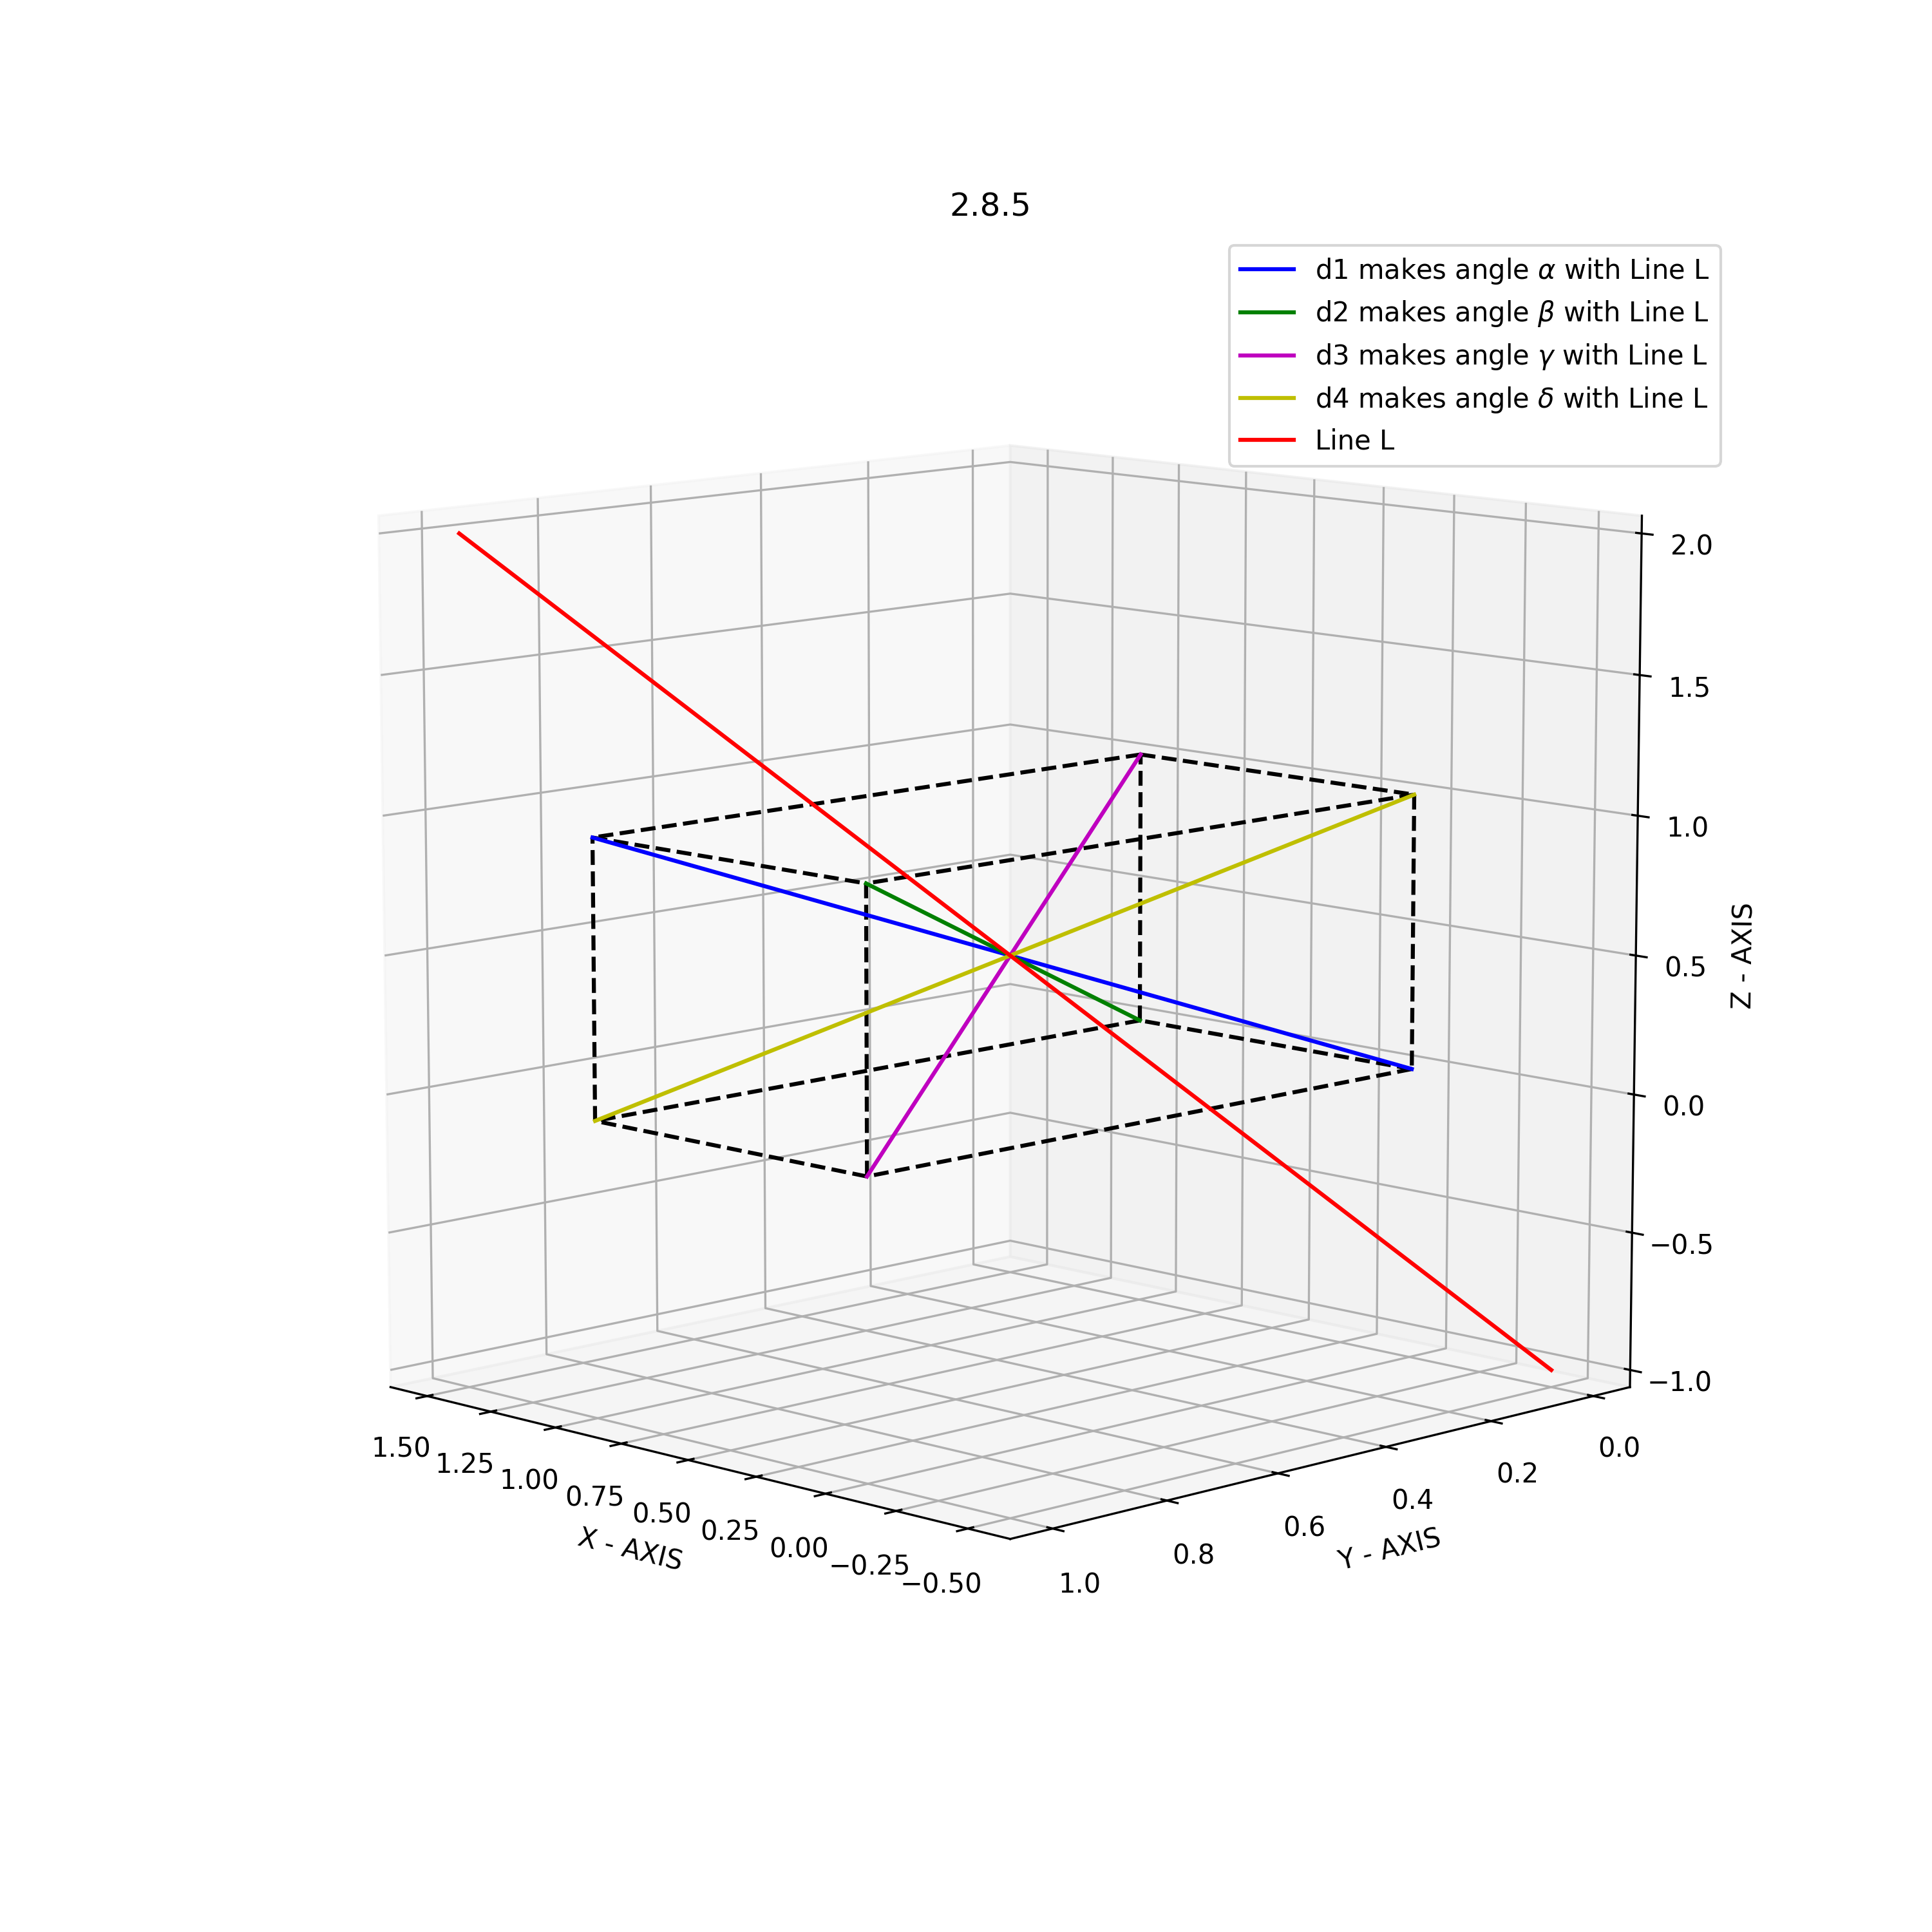
\includegraphics[width=0.7\linewidth]{figs/fig.png}
    \caption{}
    \label{fig:3DVectors}
\end{figure}
\end{frame}

\begin{frame}[fragile]{Python Code: plot.py (Native)}
\begin{lstlisting}[language=Python]
import numpy as np
import matplotlib.pyplot as plt
from mpl_toolkits.mplot3d import Axes3D

p1 = np.array([0,0,0])
p2 = np.array([1,0,0])
p3 = np.array([1,0,1])
p4 = np.array([0,0,1])
p5 = np.array([0,1,0])
p6 = np.array([1,1,0])
p7 = np.array([1,1,1])
p8 = np.array([0,1,1])

fig = plt.figure(figsize = (10,10))
ax = fig.add_subplot(111, projection = '3d')
\end{lstlisting}
\end{frame}


\begin{frame}[fragile]{Python Code (Native Implementation – plot.py)}
\begin{lstlisting}[language=Python]
# Bottom face
ax.plot([p1[0], p2[0]], [p1[1], p2[1]], [p1[2], p2[2]], 'k--')
ax.plot([p2[0], p3[0]], [p2[1], p3[1]], [p2[2], p3[2]], 'k--')
ax.plot([p3[0], p4[0]], [p3[1], p4[1]], [p3[2], p4[2]], 'k--')
ax.plot([p4[0], p1[0]], [p4[1], p1[1]], [p4[2], p1[2]], 'k--')

# Top face
ax.plot([p5[0], p6[0]], [p5[1], p6[1]], [p5[2], p6[2]], 'k--')
ax.plot([p6[0], p7[0]], [p6[1], p7[1]], [p6[2], p7[2]], 'k--')
ax.plot([p7[0], p8[0]], [p7[1], p8[1]], [p7[2], p8[2]], 'k--')
ax.plot([p8[0], p5[0]], [p8[1], p5[1]], [p8[2], p5[2]], 'k--')

# Vertical edges
ax.plot([p1[0], p5[0]], [p1[1], p5[1]], [p1[2], p5[2]], 'k--')
ax.plot([p2[0], p6[0]], [p2[1], p6[1]], [p2[2], p6[2]], 'k--')
ax.plot([p3[0], p7[0]], [p3[1], p7[1]], [p3[2], p7[2]], 'k--')
ax.plot([p4[0], p8[0]], [p4[1], p8[1]], [p4[2], p8[2]], 'k--')
\end{lstlisting}
\end{frame}

\begin{frame}[fragile]{Python Code (Native Implementation – plot.py)}
\begin{lstlisting}[language=Python]
# Body diagonal from p1 to p7
ax.plot([p1[0], p7[0]], [p1[1], p7[1]], [p1[2], p7[2]], 'b', label = r"d1 makes angle $\alpha$ with Line L")

# Body diagonal from p2 to p8
ax.plot([p2[0], p8[0]], [p2[1], p8[1]], [p2[2], p8[2]], 'g', label = r"d2 makes angle $\beta$ with Line L")

# Body diagonal from p3 to p5
ax.plot([p3[0], p5[0]], [p3[1], p5[1]], [p3[2], p5[2]], 'm', label = r"d3 makes angle $\gamma$ with Line L")

# Body diagonal from p4 to p6
ax.plot([p4[0], p6[0]], [p4[1], p6[1]], [p4[2], p6[2]], 'y', label = r"d4 makes angle $\delta$ with Line L")

# Center of the cube
center = np.array([0.5, 0.5, 0.5])

\end{lstlisting}
\end{frame}

\begin{frame}[fragile]{Python Code (Native Implementation – plot.py)}
\begin{lstlisting}[language=Python]
v = np.array([2, 1, 3]) # Direction vector of the line

k = 0.5 # Parameter for length of the line

start = center - k * v
end = center + k * v

ax.plot([start[0], end[0]], [start[1], end[1]], [start[2], end[2]], 'r', label = 'Line L')

ax.set_xlabel("X - AXIS")
ax.set_ylabel("Y - AXIS")
ax.set_zlabel("Z - AXIS")
ax.set_title("2.8.5")

ax.legend()
ax.set_box_aspect([1, 1, 1])
ax.view_init(elev=10, azim=135)
plt.savefig("fig4.png", dpi=300)
plt.show()

\end{lstlisting}
\end{frame}


\begin{frame}[fragile]{C Code (Shared Library – findcube.c)}
\begin{lstlisting}[language=C]
#include <stdio.h>

void find_cube(double n, double *dir_vec, double len_par, double *cube_pts, double *start, double *end) {
    double pts[8][3] = {
        {0, 0, 0}, {n, 0, 0}, {n, 0, n}, {0, 0, n}, // bottom face
        {0, n, 0}, {n, n, 0}, {n, n, n}, {0, n, n}  // top face
    };

    for (int i = 0; i < 8; i++) {
        for (int j = 0; j < 3; j++) {
            cube_pts[i*3 + j] = pts[i][j];
        }
    }

    double center[3] = { n/2, n/2, n/2 };
\end{lstlisting}
\end{frame}

\begin{frame}[fragile]{C Code (Shared Library – findprojection.c)}
\begin{lstlisting}[language=C]
    for (int i = 0; i < 3; i++) {
        start[i] = center[i] - len_par * dir_vec[i];
        end[i]   = center[i] + len_par * dir_vec[i];
    }
}
\end{lstlisting}
\end{frame}


\begin{frame}[fragile]{Python Code (C Integrated – call.py)
}
\begin{lstlisting}[language=Python]
import ctypes
import numpy as np
import matplotlib.pyplot as plt
from mpl_toolkits.mplot3d import Axes3D

so = ctypes.CDLL("./find_cube.so")

so.find_cube.argtypes = [
    ctypes.c_double,
    ctypes.POINTER(ctypes.c_double),
    ctypes.c_double,
    ctypes.POINTER(ctypes.c_double),
    ctypes.POINTER(ctypes.c_double)
]
so.find_cube.restype = None

n = 1.0
dir_vec = np.array([2, 1, 3], dtype=np.double)
dir_vec_ptr = dir_vec.ctypes.data_as(ctypes.POINTER(ctypes.c_double))
len_par = 0.5
\end{lstlisting}
\end{frame}

\begin{frame}[fragile]{Python Code (C Integrated – call.py)
}
\begin{lstlisting}[language=Python]
cube_pts = (ctypes.c_double*24)()  # 8 points × 3 coords
start_arr = (ctypes.c_double*3)()
end_arr = (ctypes.c_double*3)()

so.find_cube(n, dir_vec_ptr, len_par, cube_pts, start_arr, end_arr)

cube_pts_np = np.array(cube_pts).reshape(8,3)
start = np.array(start_arr)
end = np.array(end_arr)

fig = plt.figure(figsize=(10,10))
ax = fig.add_subplot(111, projection='3d')

edges_idx = [
    (0,1),(1,2),(2,3),(3,0),  # bottom
    (4,5),(5,6),(6,7),(7,4),  # top
    (0,4),(1,5),(2,6),(3,7)   # vertical
]
\end{lstlisting}
\end{frame}

\begin{frame}[fragile]{Python Code (C Integrated – call.py)
}
\begin{lstlisting}[language=Python]
for i,j in edges_idx:
    s = cube_pts_np[i]
    e = cube_pts_np[j]
    ax.plot([s[0],e[0]], [s[1],e[1]], [s[2],e[2]], 'k--')

body_diags_idx = [(0,6),(1,7),(2,4),(3,5)]
colors = ['b','g','m','y']
labels = ['d1','d2','d3','d4']

for (i,j),color,label in zip(body_diags_idx,colors,labels):
    s = cube_pts_np[i]
    e = cube_pts_np[j]
    ax.plot([s[0],e[0]], [s[1],e[1]], [s[2],e[2]], color=color, label=label)

ax.plot([start[0],end[0]], [start[1],end[1]], [start[2],end[2]], 'r', label='Line L')
\end{lstlisting}
\end{frame}

\begin{frame}[fragile]{Python Code (C Integrated – call.py)
}
\begin{lstlisting}[language=Python]
ax.set_xlabel("X - AXIS")
ax.set_ylabel("Y - AXIS")
ax.set_zlabel("Z - AXIS")
ax.set_title(r"Line L making angles $\alpha, \beta, \gamma, \delta$ with the body diagonals of a cube")
ax.legend()
ax.set_box_aspect([1,1,1])
ax.view_init(elev=10, azim=135)

plt.savefig("fig_cube_line.png", dpi=300)
plt.show()
\end{lstlisting}
\end{frame}

\end{document}